
\chapter{Arquitetura de Software}
\label{sec-arquitetura}

A arquitetura de software do sistema~\imprimirtitulo  segue a arquitetura padrão sugerida pelo FrameWeb~\cite{souza:masterthesis07,souza-et-al:iism09} baseada no padrão Camada de Serviço~\cite{fowler:book02}. A Figura~\ref{figura-arquitetura-padrao} ilustra a arquitetura e indica onde atuam os \textit{frameworks} para o desenvolvimento Web, listados na Tabela~\ref{tabela-plataforma}.

\begin{figure}[h]
	\centering
	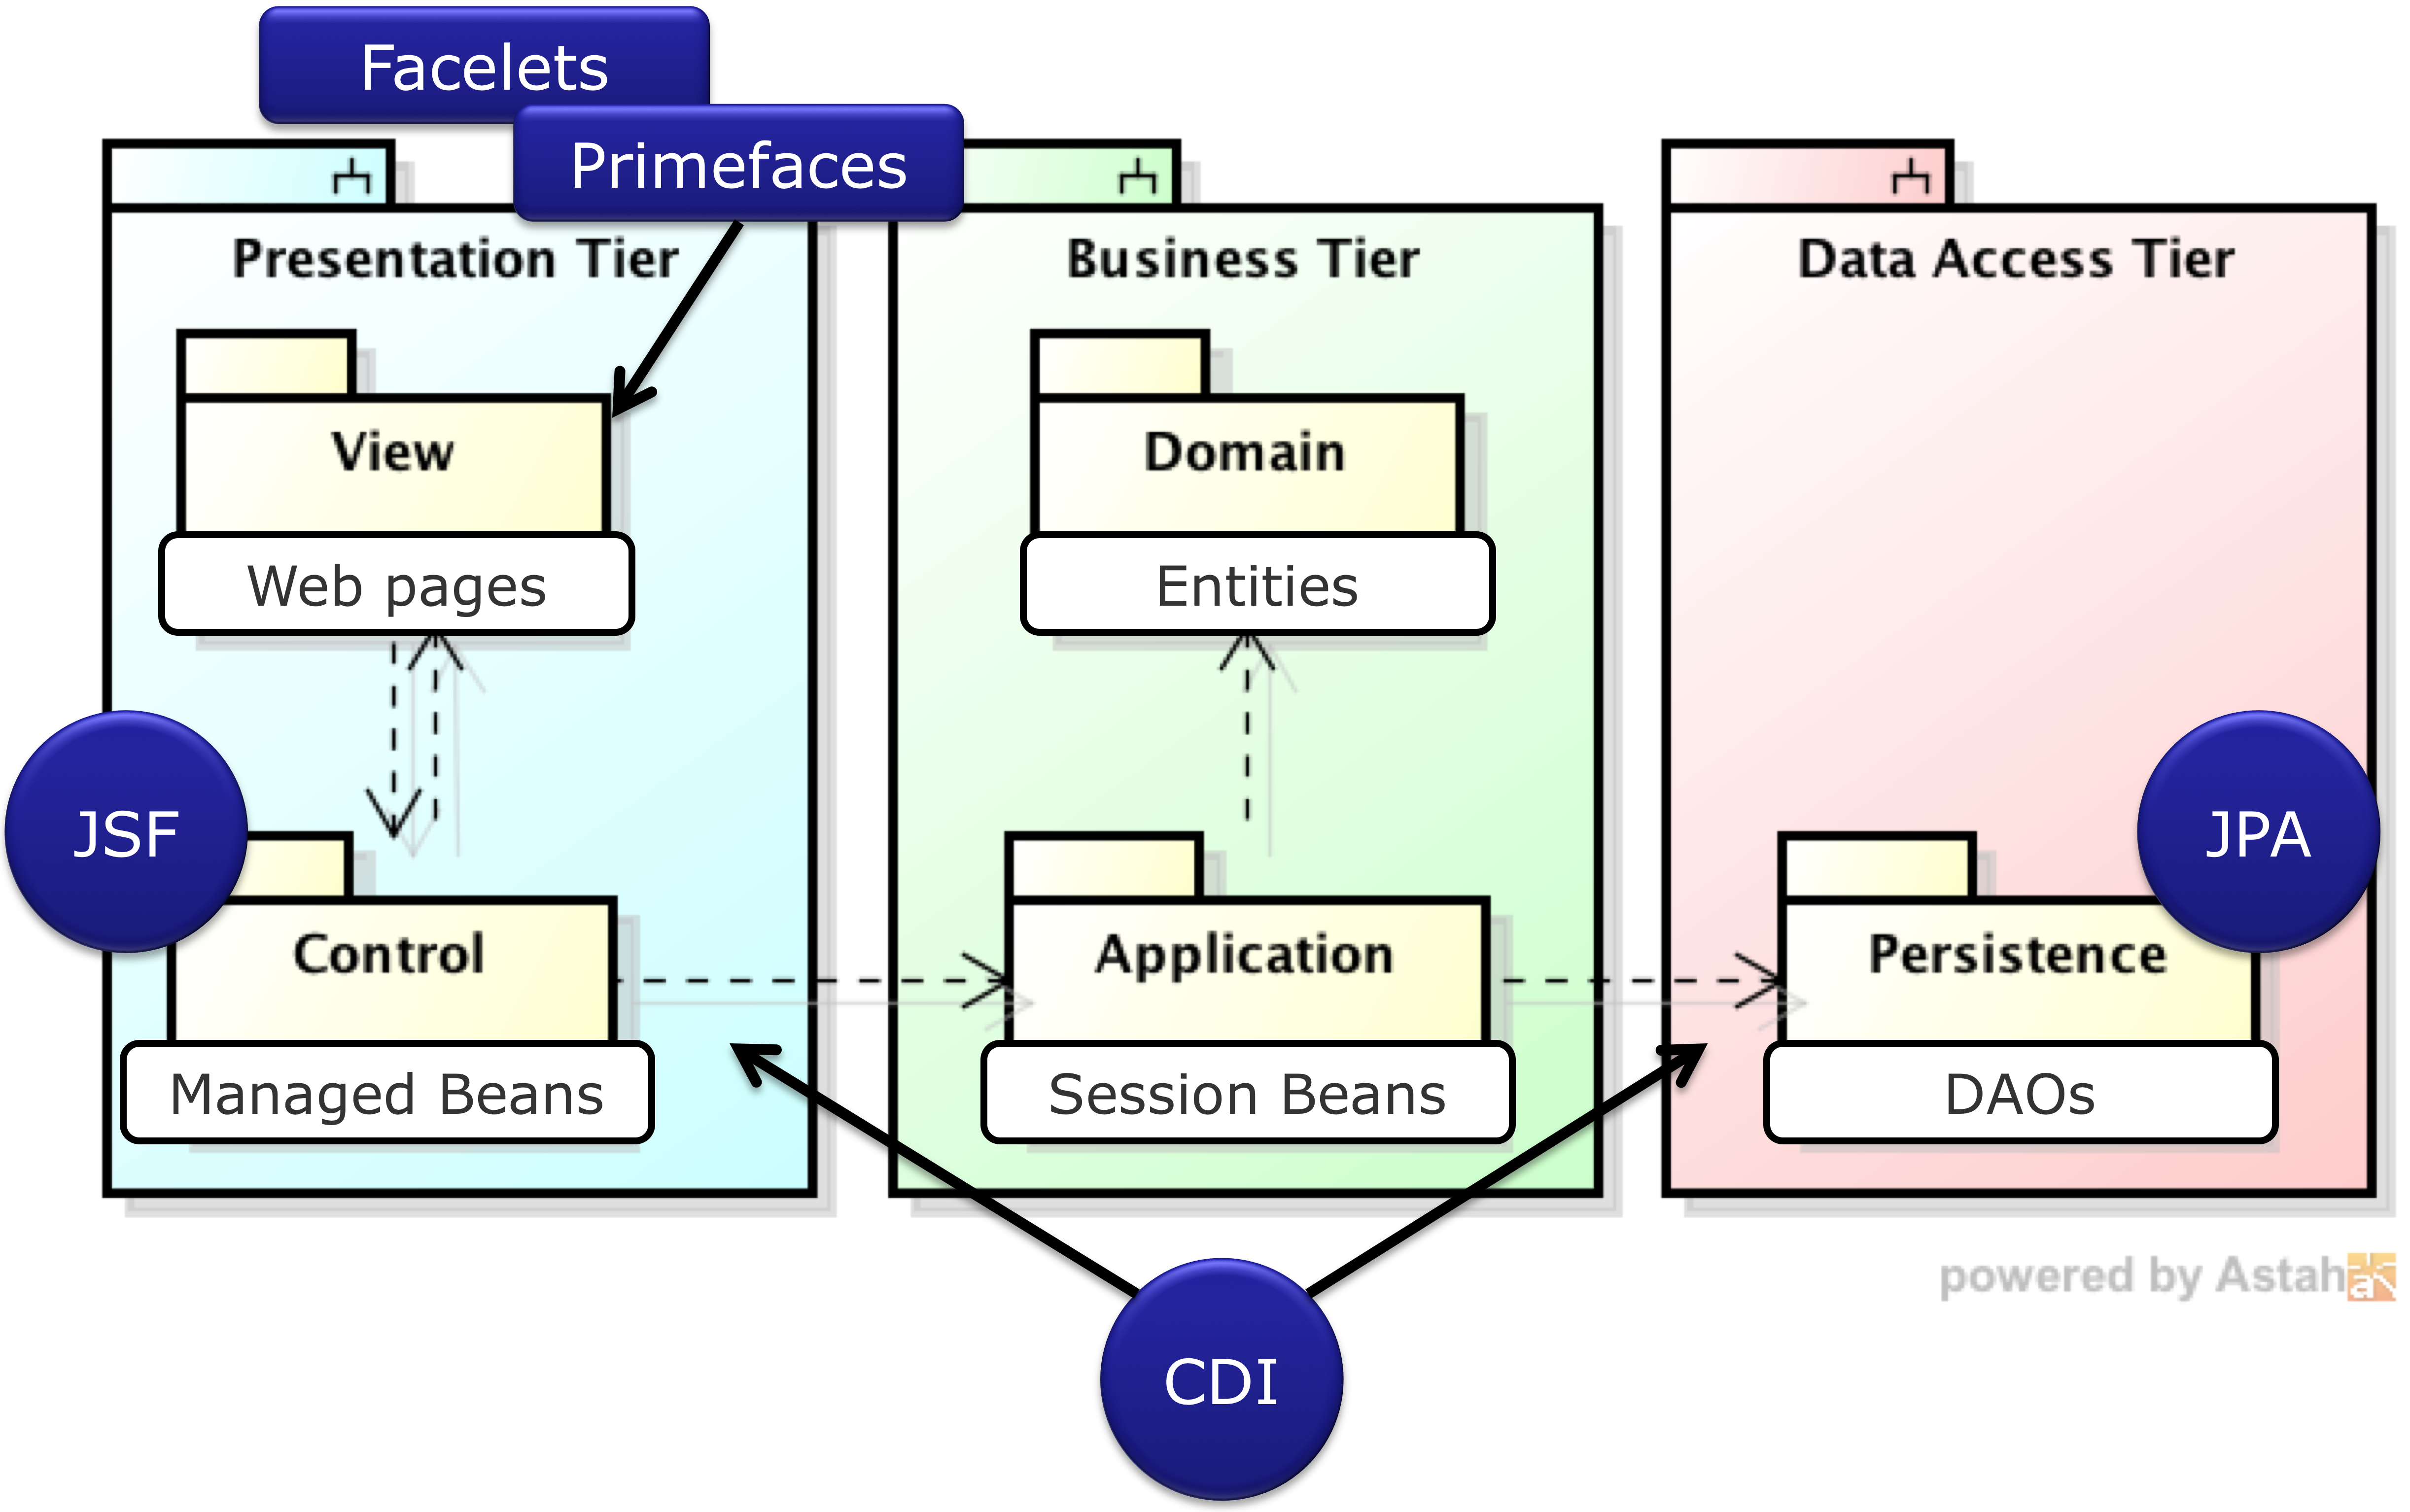
\includegraphics[width=0.8\textwidth]{figuras/figura-arquitetura-padrao.png}
	\caption{Arquitetura padrão proposta pelo FrameWeb.}
	\label{figura-arquitetura-padrao}
\end{figure}

Nas próximas seções, serão apresentados diagramas FrameWeb relativos a cada uma das camadas da arquitetura do sistema.

Alguns desses diagramas possuem algumas inconsistências decorrentes de pequenos problemas na ferramenta de edição utilizada.

\begin{itemize}

\item Uma das inconsistências trata-se dos tipos de dados genéricos nos atributos e nos métodos presentes nos diagramas. Não é possível na versão atual especificar o tipo de objeto presente nas coleções. \footnote{\url{https://github.com/nemo-ufes/FrameWeb/issues/5}}

\item Uma outra inconsistência se refere à cardinalidade em um relacionamento entre página e formulário. Não é possível especificar, na versão atual do editor, a cardinalidade de uma associação de navegação.\footnote{\url{https://github.com/nemo-ufes/FrameWeb/issues/6}}

\end{itemize}

Por fim, em alguns modelos de navegação, o controlador apresenta atributos que não são nem fornecidos como parâmetro a um dos métodos, nem obtidos do serviço. Estes casos devem-se a elementos não apresentados na presente versão deste documento, que não apresenta o sistema completo, mas apenas, visando cumprimento de prazos, apenas atende as exigências da atividade 1 de preparação do trabalho. A intenção é que alguns elementos como por exemplo \textit{aluno} no modelo de navegação de solicitação de matrícula, ou \textit{professor} no modelo de navegação de gerenciamento de solicitações de matrícula, estarão disponíveis na sessão do usuário, imediatamente após o \textit{login}.

\section{Camada de Apresentação}
\label{sec-arquitetura-apresentacao}



A Figura~\ref{navegacao-solicitar-matricula-10} mostra o modelo de navegação para a funcionalidade Solicitar Matrícula, que é realizada pelo aluno a partir do momento em que ele se encontra habilitado para cursar as disciplinas. Esta habilitação ocorre no momento em que uma pessoa (candidato) é aprovada na seleção, é aceita por um orientador a fim de iniciar no curso, e se comunica a secretaria do curso sobre o fato para a realização da matrícula no curso.

\begin{figure}[h]
	\centering
	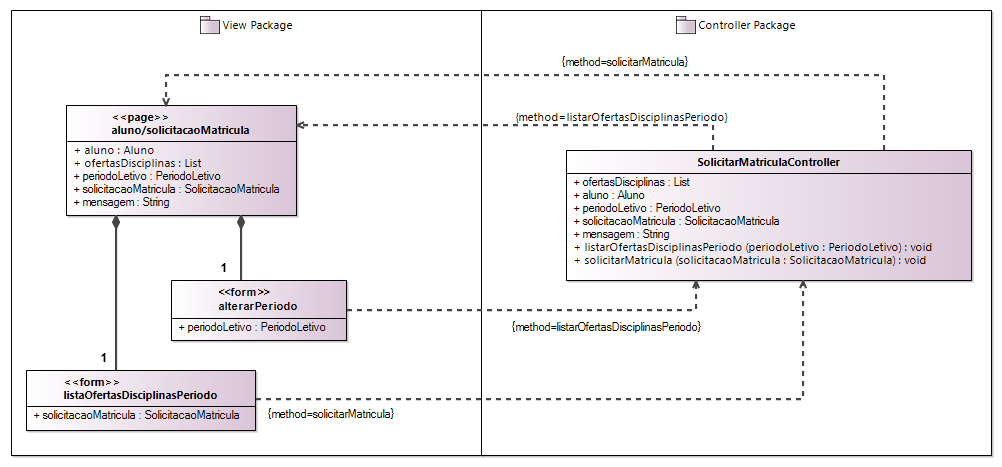
\includegraphics[width=0.8\textwidth]{figuras/navegacao-solicitar-matricula-10.png}
	\caption{Modelo de Navegação Solicitar Matrícula.}
	\label{navegacao-solicitar-matricula-10}
\end{figure}

A Figura~\ref{navegacao-gerenciar-solicitacoes-matricula-10} mostra o modelo de navegação para a funcionalidade onde o orientador avalia as solicitações de matrículas recebidas pelos alunos e fornece um parecer.

\begin{figure}[h]
	\centering
	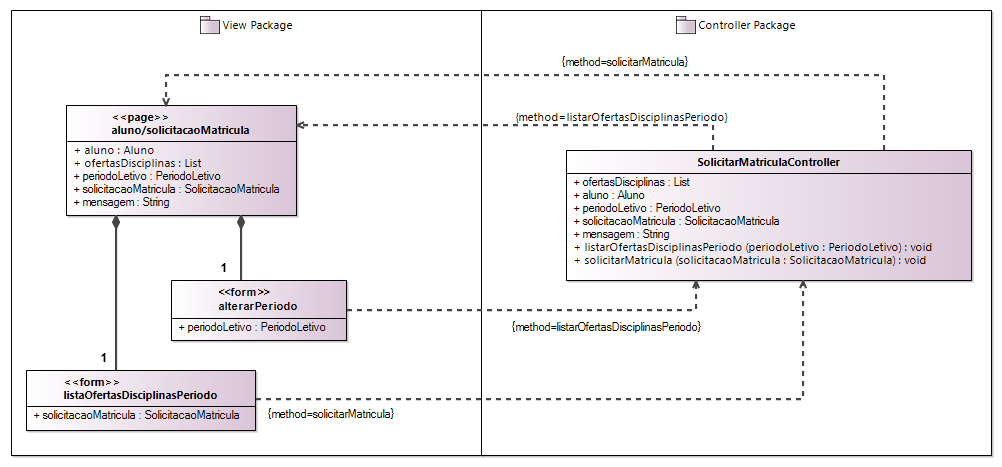
\includegraphics[width=0.8\textwidth]{figuras/navegacao-solicitar-matricula-10.png}
	\caption{Modelo de Navegação Gerenciar Solicitações de Matrícula.}
	\label{navegacao-gerenciar-solicitacoes-matricula-10}
\end{figure}

A Figura~\ref{navegacao-gerenciar-candidatos-10} mostra o modelo de navegação para as funcionalidades referentes ao cadastro dos candidatos aprovados no processo de seleção.

\begin{figure}[h]
	\centering
	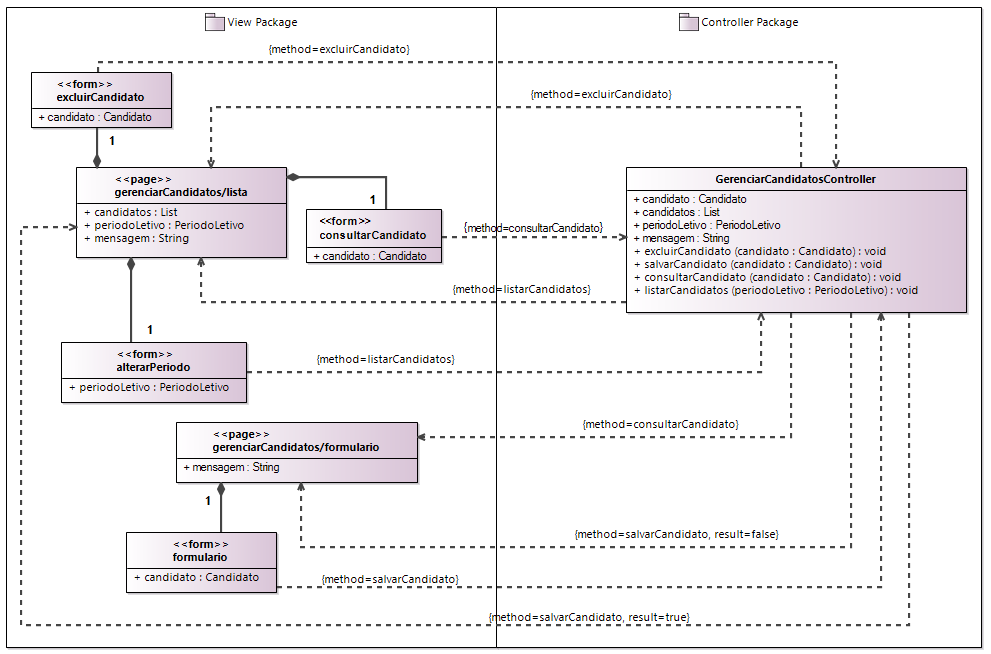
\includegraphics[width=0.8\textwidth]{figuras/navegacao-gerenciar-candidatos-10.png}
	\caption{Modelo de Navegação Gerenciar Candidatos.}
	\label{navegacao-gerenciar-candidatos-10}
\end{figure}



\section{Camada de Negócio}
\label{sec-arquitetura-negocio}

A Figura~\ref{modelo-entidades-10} exibe o modelo de entidades do sistema.

\begin{figure}[h]
	\centering
	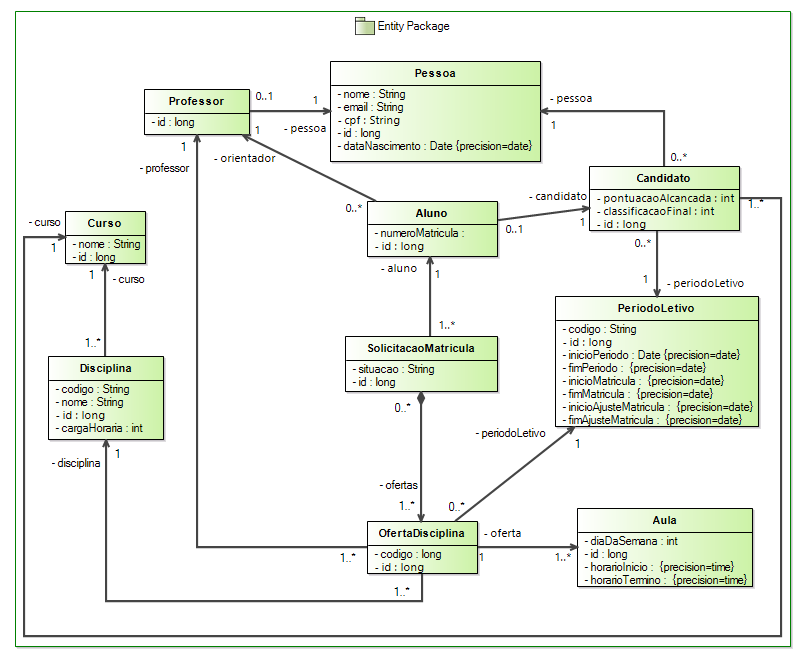
\includegraphics[width=0.8\textwidth]{figuras/modelo-entidades-10.png}
	\caption{Modelo de Entidades.}
	\label{modelo-entidades-10}
\end{figure}

A Figura~\ref{modelo-aplicacao-10} exibe o modelo de aplicação demonstrando as dependências entre os componentes da arquitetura.

\begin{figure}[h]
	\centering
	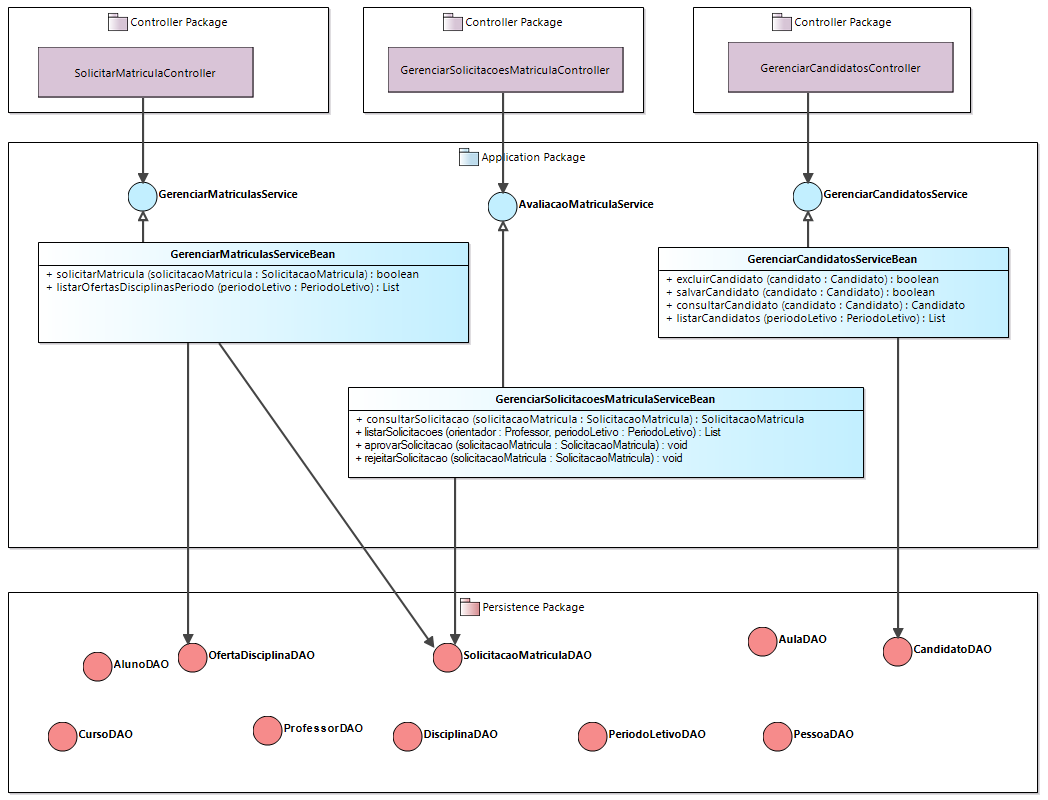
\includegraphics[width=0.8\textwidth]{figuras/modelo-aplicacao-10.png}
	\caption{Modelo de Aplicação.}
	\label{modelo-aplicacao-10}
\end{figure}

\section{Camada de Acesso a Dados}
\label{sec-arquitetura-dados}

A Figura~\ref{modelo-persistencia-10} exibe o modelo de persistência do sistema.

\begin{figure}[h]
	\centering
	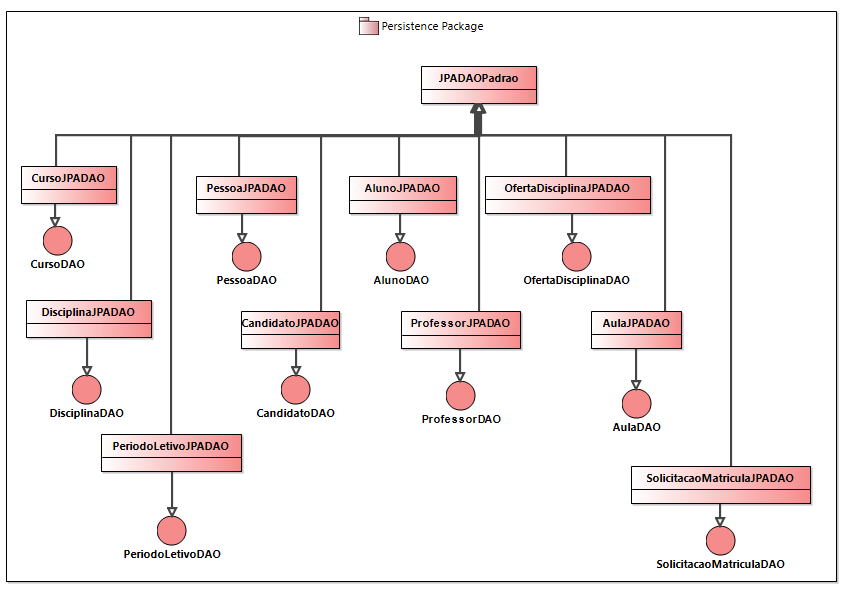
\includegraphics[width=0.8\textwidth]{figuras/modelo-persistencia-10.png}
	\caption{Modelo de Persistência}
	\label{modelo-persistencia-10}
\end{figure}


